\newpage
\section{Testing}
\label{sec:Testing}
Tijdens de realisatieperiode wordt er gebruikgemaakt van de V-Model.
Het V-Model \ref{fig:VModel} toont dat er voor de verschillende design lagen van het systeem verschillende testen gebruikt worden.
De verschillende units/modules van code worden getest door middel van unit testing.
Vervolgens worden de samen hangende units/modules getest door integratie testen om het softwaredesign te kunnen valideren.
De laag boven softwaredesign is systeemanalyse, dit wordt getest door middel van systeem testing.
Daarna worden de requirements gevalideerd door acceptatie testen uit te voeren met de stakeholders. \\
\begin{graphic}
    \vspace{0.2cm}
    \captionsetup{type=figure}
    \caption{V-Model \Parencite{VModel}}
    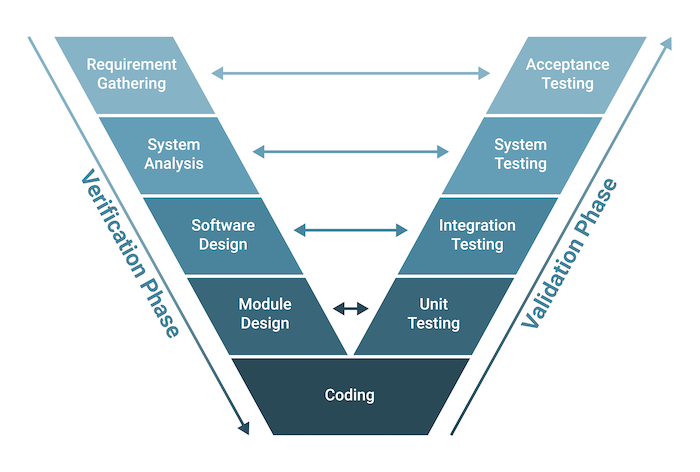
\includegraphics[scale=0.4]{VModel}
    \label{fig:VModel}
    \vspace{0.2cm}
\end{graphic}
